\documentclass[noindent,nohyp,parspace,titlepage,twoside,12pt]{article}

\usepackage{adjustbox}
\usepackage{algorithm}
\usepackage{algpseudocode}
\usepackage{amsfonts}
\usepackage{amsmath}
\usepackage[backend=biber,sorting=none]{biblatex}
% \usepackage[type={CC},modifier={by-sa},version={4.0}]{doclicense}
\usepackage{geometry}
\usepackage{hyperref}
\usepackage{listings}
\usepackage{pgfplots}
\usepackage{xparse}

\addbibresource{thesis.bib}

\usetikzlibrary{shapes,matrix}

\graphicspath{{img/}}

\hypersetup{
  colorlinks,
  citecolor=black,
  filecolor=black,
  linkcolor=black,
  urlcolor=black
}

\pgfplotsset{compat=1.18}
\setcounter{secnumdepth}{5}
\setcounter{tocdepth}{5}

\def\TITLE{\
  Investigating Bias \\
  in LLM Self-Evaluation\
}
\def\AUTHOR{Attila M. Magyar}

\title{\TITLE}
\author{\AUTHOR}

\linespread{1.25}
\begin{document}

\begin{titlepage}

  \begin{center}
    \Huge\textbf{\TITLE}\normalsize
  \end{center}
  \begin{center}
    \Large Thesis \normalsize
  \end{center}

  \vfill

% TODO: author, supervisor

  \vfill

  \begin{center}
    \Large Mathematics Expert in Data Analytics and Machine Learning
    \normalsize
  \end{center}

  \begin{center}
    
\includegraphics[scale=0.2]{img/logo.png} \\
  \end{center}

  \begin{center}
    \Large Eötvös Loránd University \\
    \Large Faculty of Science \normalsize
  \end{center}

  \begin{center}
    \Large Budapest, 2025 \normalsize
  \end{center}

\end{titlepage}

  \tableofcontents

\newpage

  \section*{Abstract}
  \addcontentsline{toc}{section}{\protect\numberline{}Abstract}

    This thesis explores whether large language models (LLMs) tend to
    overestimate the quality of their own outputs when serving as judges or
    evaluators. Preliminary observations suggest that using the same or
    closely related LLM as both generator and judge may inflate performance
    metrics. Through systematic experiments, the project will quantify this
    potential bias and discuss its implications for AI evaluation, fairness,
    and trustworthiness in model benchmarking.

  \section{Introduction}

    This section introduces the key terms and core concepts that will be used
    in later sections.

    \subsection{A Brief Introduction to LLMs}

      A language model is a machine learning model designed to perform a wide
      range of tasks that involve natural language processing (NLP), including
      text summarization, translation, sentiment analysis, spam detection,
      content moderation, text generation, etc.

      Significant advancements in deep learning \cite{attention,gpt3,gpt4} led
      to the emergence of \textbf{large language models} (LLMs) --- particularly
      generative LLMs --- which in the early 2020s became commercialized and
      widely adopted in both industry and popular discourse.

      A generative LLM is a model which has a parameter count on the order of
      billions or more (hence "large"), and predicts the conditional
      probability \cite{llms}

      \begin{align} \label{eqautoreg}
        P(w_m | w_0, \cdots, w_{m-1})
      \end{align}

      where $m \in \mathbb{N}$, $w_0$ is a special start symbol, and $w_k$ is
      the $k$-th token (for $1 \le k \le m$) in a sequence of tokens that form
      a piece of text in some language, be it a natural language or a formal
      one like programming languages. The interpretation of the tokens depends
      on the exact tokenization strategy used, which may define tokens as
      words, word pieces, n-grams, or individual characters, and spaces,
      punctuation marks, etc.

      \textbf{Encoding} is the process which converts human-readable textual
      tokens into integers which uniquely identify each token within the
      predetermined vocabulary of the model, and the inverse of this mapping
      is called \textbf{decoding}. \footnote{Internally, the token numbers are
      mapped by a trainable model to vectors within a vector space called the
      \textbf{embedding space}. The choice for the dimensionality of this space
      allows a significant dimensionality reduction compared to what would be
      necessary for example to represent the tokens with one-hot encoding. An
      interesting property of the embedding space is that it tends to map
      tokens that are close to each other in meaning to vectors which are close
      to each other in the space.}

      Text generation is an autoregressive process where given a
      sequence of tokens as a prefix --- known as the \textbf{prompt} --- the
      model estimates the probability distribution of the next token, takes a
      sample from that distribution, appends it to the sequence, and repeats
      the process with the extended sequence until a stopping condition is met.

      A frequently used parameter to control the sampling is called the
      \textbf{temperature} \cite{temperature}: the closer it is to 0, the more
      the sampling will lean toward the most probable token --- making the
      algorithm more deterministic ---, while higher values increase the
      randomization, making the generated text feel more \emph{creative} until,
      above a certain threshold, it becomes incoherent and semantically
      meaningless. \footnote{If $v \in \mathbb{N}$ denotes the number of all
      possible tokens available for the model (vocabulary size), and
      $\mathbf{s} \in \mathbb{R}^v$ is an output vector of the model assigning
      a score to each token as the continuation of a given input, then the
      distribution for the sampling, with respect to the temperature $T \in
      \mathbb{R}$ can be calculated via the softmax function:
      $\text{softmax}\left(\frac{1}{T} \mathbf{s}\right) = \left[
      \frac{\exp(\frac{s_i}{T})}{\sum_{j=1}^v \exp(\frac{s_j}{T})}
      \right]_{i=1}^v$} In practical implementations, if $T$ is sufficiently
      close or exactly equal to $0$, then the sampling is usually replaced with
      the deterministic argmax function in order to preserve numerical
      stability.  Non-zero $T$ values control the flatness of the distribution,
      leading to the aforementioned behavior.

      \begin{figure}[hbtp]
        \label{figtemperature}
        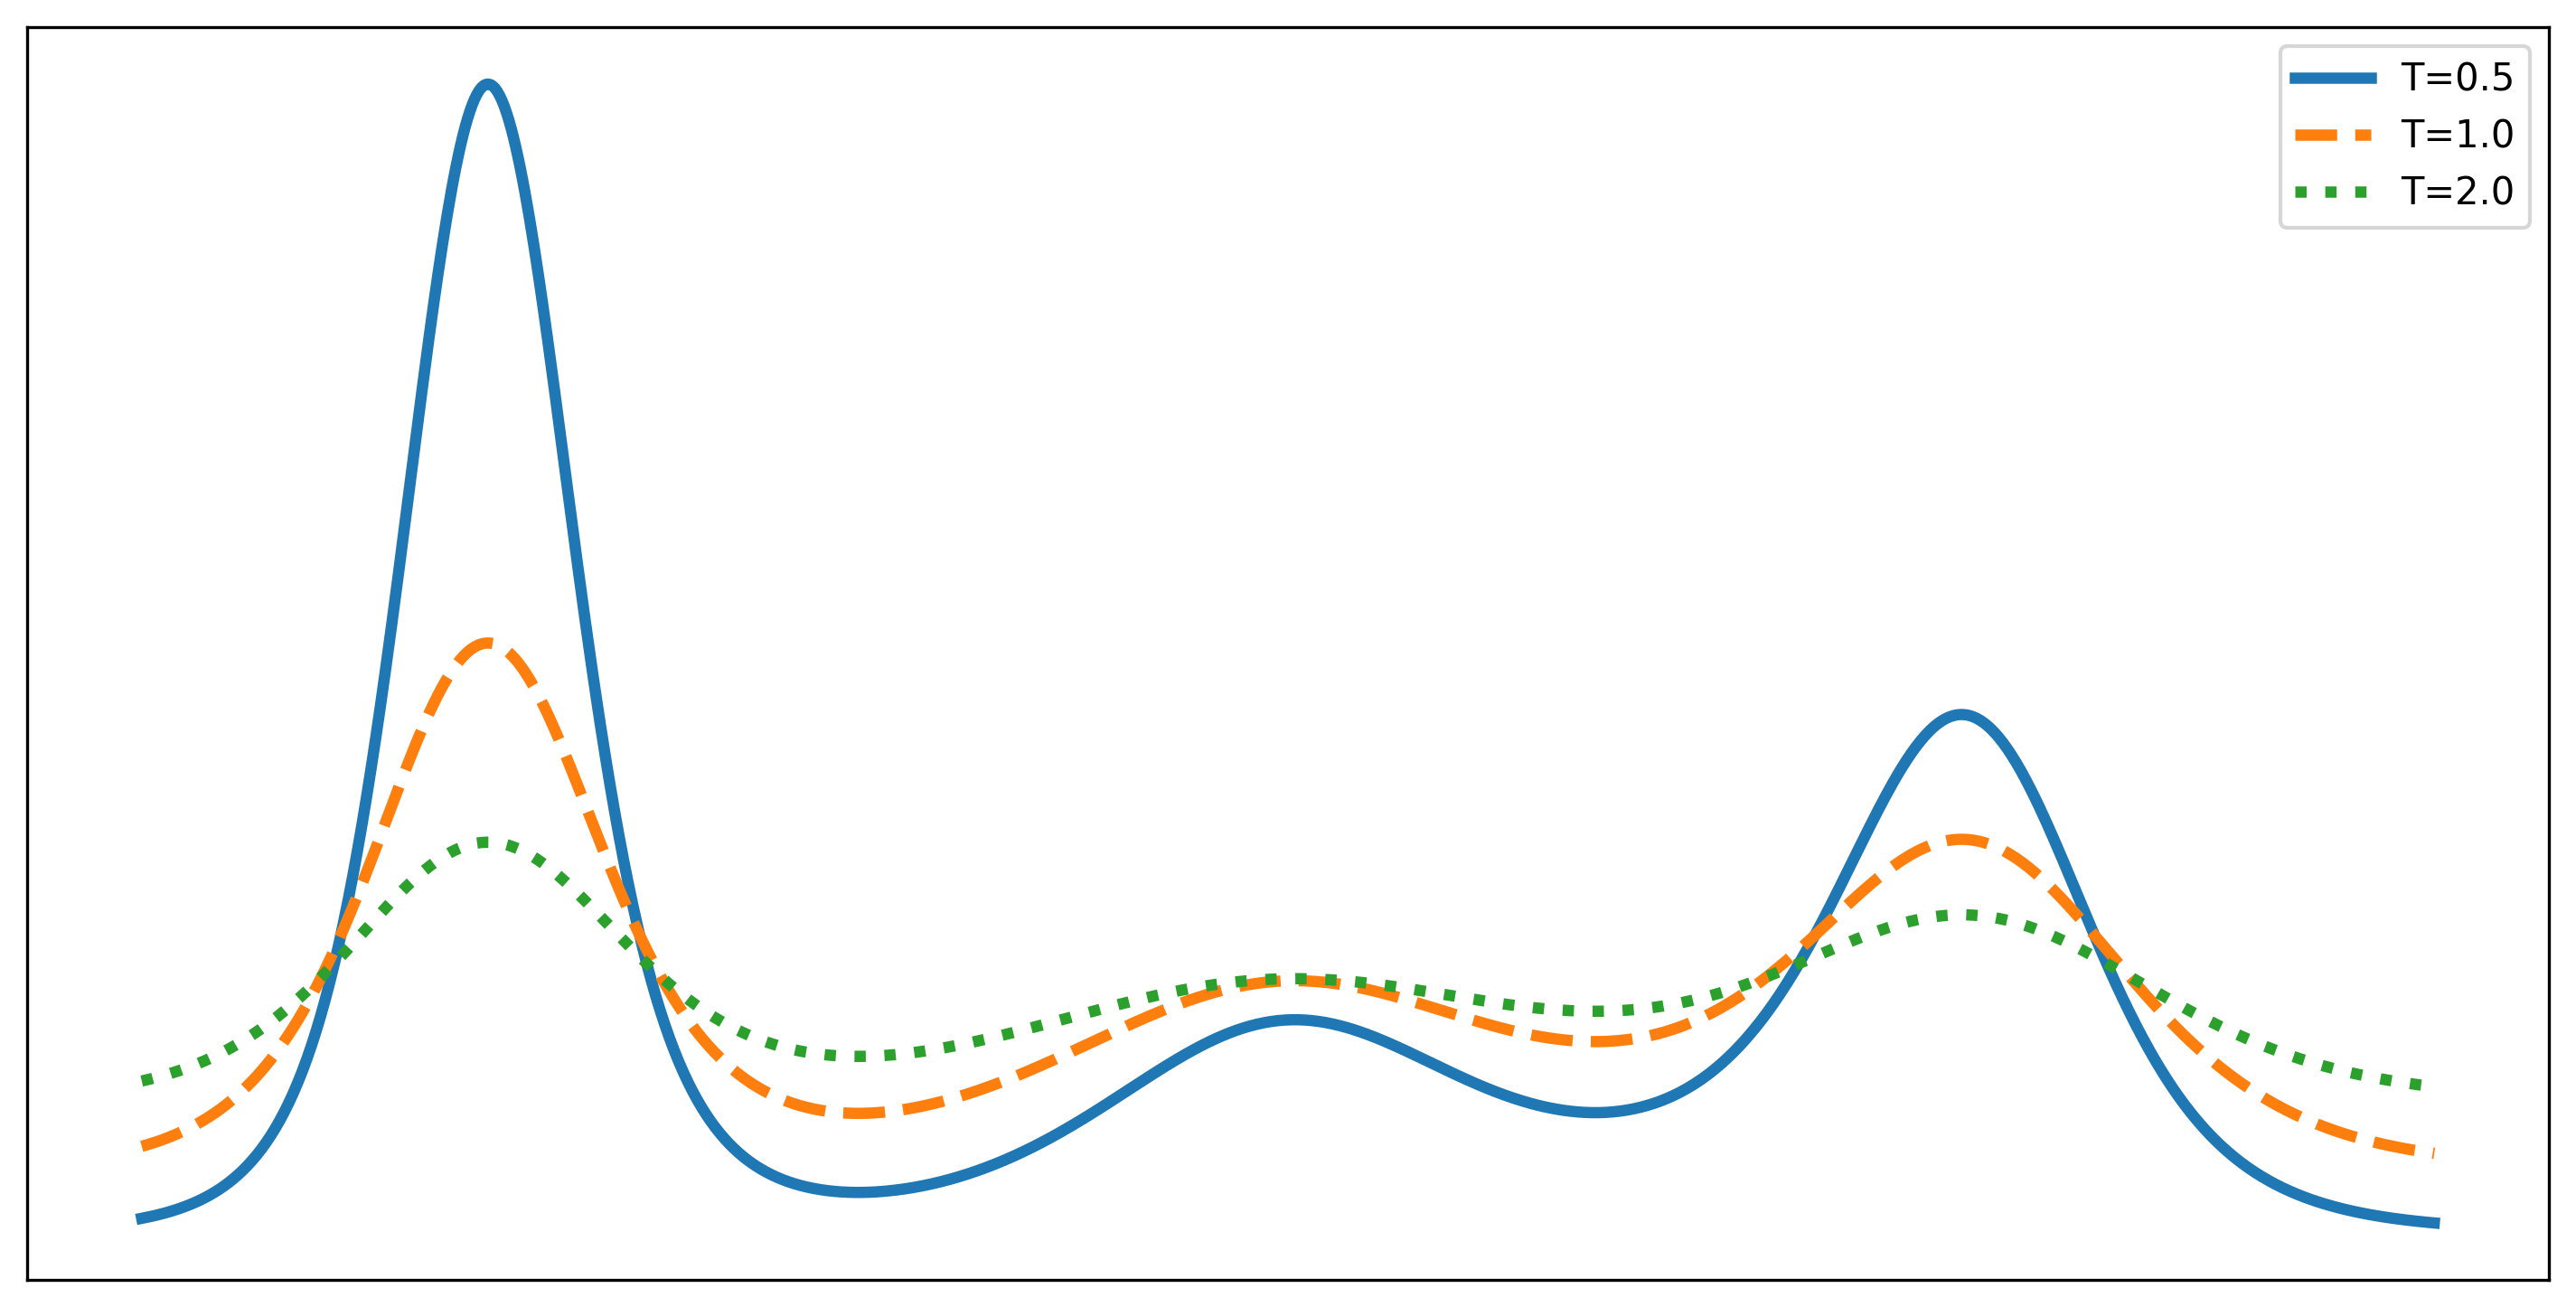
\includegraphics[width=\textwidth]{softmax-temperature}
        \caption{Effect of the temperature parameter on token probabilities.}
      \end{figure}

      With sufficiently large model complexity and training corpora size and
      diversity, LLMs start to exhibit capabilities which rival that of top
      performer humans in a broad class of problems \cite{gpt3,gpt4}. The
      versatility of the models is often utilized in a setting where the prompt
      is composed of two parts, each consisting of instructions given in
      natural language:

      \begin{itemize}
        \item the \textbf{system prompt} can instruct the model to behave in a
              certain way, for example, to act like a helpful AI assistant,
              an expert in a domain, or to generate its texts in the style of
              fictional 18th-century Caribbean pirates, etc.

        \item and the \textbf{user prompt} which describes the task to be
              carried out by the model, ranging from text translation or
              summarization to solving complex programming problems or pointing
              out business risks in legal documents, and more.
      \end{itemize}

      Generative models with sufficient generalization capabilities can predict
      likely continuations of such prompts with such high accuracy that as an
      emergent phenomenon, the generated text will often contain an actual
      solution to the proposed problem. This instruction-following paradigm
      enables models to perform \textbf{few-shot learning} \cite{gpt3} or even
      \textbf{zero-shot learning} by interpreting tasks directly from the
      natural language description, based on just a few or zero examples,
      respectively, without specific training or fine-tuning.

      The problem solving performance of LLMs can be improved further by
      prompt engineering techniques like \textbf{chain-of-thought} prompting
      \cite{cot}, where the model is provided with step-by-step example
      solutions to related problems in the prompt, encouraging it to also
      articulate intermediate reasoning steps before arriving at its final
      answer. It is worth emphasizing that --- recalling formula
      \ref{eqautoreg} and the autoregressive text generation process --- the
      chain-of-thought is only effective if it is placed \emph{before} the
      final answer.

    \subsection{LLM Evaluators, LLM-as-a-Judge}

      The continuing development of LLMs and their integration into more and
      more systems to support a growing number of use cases necessitates regular
      measurement of their capabilities and monitoring their alignment with
      human preferences.

      While evaluating the quality of LLM-generated text by utilizing human
      labor does not scale well, may suffer from human error or subjective
      personal preference bias, and can be expensive, traditional algorithmic
      metrics which often rely on surface-level similarities to reference
      examples (like BLEU for machine translation \cite{bleu} or ROUGE for
      summarization and translation \cite{rouge}), often fall short of achieving
      acceptable correlation levels with human judgement.

      In recent years, in order to overcome these problems, the
      \textbf{LLM-based evaluation} or \textbf{LLM-as-a-judge} paradigm has
      been proposed \cite{gptscore,chatgptgoodeval,reffree,geval},
      where --- taking advantage of the instruction following and the zero-shot
      and few-shot learning capabilities of LLMs --- a model is instructed to
      act as a fair judge and generate a quality assessment for a piece of
      generated text either in the form of a single score, or one accompanied by
      an explanation or a list of problems. An advantage of the latter approach
      --- besides easier interpretability --- is that enumerating evidences
      before giving a final result can influence the score via the
      autoregressive generation process, similarly to the improvements achieved
      by making large models include a chain-of-thought \cite{cot} breakdown of
      complex problems before the final answer.

      \subsubsection{LLM-Judge Prompting Basics}

        There are numerous strategies to implement LLM-judges in practice
        \cite{judgetaxonomy}, but a robust LLM-judge prompt usually includes
        the following elements:

        \begin{itemize}
          \item \textbf{Instructions} which clearly specify the evaluation task.

          \item Evaluation \textbf{aspects}, e.g. clarity, consistency,
                coherence, factuality, fluency, grammaticality,
                informativeness, structure, understandability, etc.

          \item Scoring \textbf{criteria} to specify the definitions for each
                score or score range.

          \item \textbf{Output format} specification so that the output of the
                judge can be programmatically parsed and interpreted.

          \item The \textbf{sample} itself to be evaluated or a pair of samples
                to be compared against each other.
        \end{itemize}

        Depending on the chosen evaluation strategy and aspect, additional
        elements may be included as well:

        \begin{itemize}
          \item Human-annotated \textbf{example} samples and their associated
                scores in few-shot evaluation scenarios.

          \item A \textbf{reference} answer for comparison with the evaluated
                sample, e.g. a human expert made translation, text summary,
                trivia answer, etc.

          \item The \textbf{source} data from which the evaluation sample was
                derived. (The original text to be translated, summarized, or
                the question to be answered, etc.)

          \item \textbf{Guidelines}, for example to help an LLM resolve the
                confusion that may arise in reference answer-based evaluations
                where some of the provided reference answers seem to contradict
                the model's own knowledge, e.g. "\emph{Don't worry
                about factuality with respect to the real world, just judge the
                example based on what you see.  No need to overthink this task,
                it really comes down to just soft matching.}" \cite{juries}.
        \end{itemize}

        \begin{figure}[hbtp]
          \label{figprompt}
          \begin{lstlisting}[frame=single,linewidth=\textwidth,basicstyle=\scriptsize]
Please act as an impartial judge and evaluate the quality of the response provided
by an AI assistant to the user question displayed below. Your evaluation should
consider factors such as the helpfulness, relevance, accuracy, depth, creativity,
and level of detail of the response. Begin your evaluation by providing a short
explanation. Be as objective as possible. After providing your explanation, please
rate the response on a scale of 1 to 10 by strictly following this format:
"[[rating]]", for example: "Rating: [[5]]".
          \end{lstlisting}
          \begin{lstlisting}[frame=single,linewidth=\textwidth,basicstyle=\scriptsize]
[Question]
{question}

[The Start of Assistant's Answer]
{answer}
[The End of Assistant's Answer]
          \end{lstlisting}
          \caption{%
            System prompt with chain-of-thought and user prompt template for an
            LLM-judge \cite{arena}.
          }
        \end{figure}

        Constructing the prompt template for a consistent, reproducible, and
        unbiased LLM-judge which also aligns well with human preferences is
        usually an iterative process, where the prompt is refined step-by-step
        until the LLM-judge can reliably produce evaluations that are
        sufficiently close to a set of human-labeled examples.

        The juding model may also be fine-tuned using evaluation data
        constructed either manually or with the assistance of advanced models
        like GPT-4.

      \subsubsection{Metrics}

        Popular choices for scoring strategy include:

        \begin{itemize}
          \item \textbf{Binary classification}: the judge is expected to
                provide a "\emph{yes}" vs. "\emph{no}", or a $0$ vs. $1$
                verdict.

          \item \textbf{Pairwise comparison}: the judge is given two candidate
                answers, and has to select the one that is a better fit for the
                evaluation criteria. \footnote{This strategy can be generalized
                as \textbf{listwise comparison} where the judge is asked to
                select the best candidate among 3 or more candidates.}
                Optionally, the judge may be allowed to declare a tie.

          \item \textbf{Multiclass classification}: the judge has to place the
                candidate on a discrete scale, usually between 1 and 5 points
                where 1 is the worst and 5 is the best.

          \item \textbf{Likert-style}: the judge has to rank the candidate
                answer along multiple dimensions using discrete scores, usually
                between 1 and 3 points where a higher score is better, then
                provide an overall 1 to 5 rating based on these scores.

          \item \textbf{Continuous score}: the candidate answer is scored with
                a number between 0 and 100.
        \end{itemize}

        If the judge LLM's interface makes the raw token probabilities
        available, then they can be used for refining discrete scores and
        making them into continuous ones by taking the sum of the discrete
        score values weighted by the probabilities of the respective tokens, as
        seen in the \textsc{G-Eval} framework \cite{geval}:

        \begin{align}
          \text{score} = \sum_{i=1}^n p(s_i) \times s_i
        \end{align}

        where $S = \{s_1, s_2, \ldots, s_n\}$ is the set of scores predefined
        in the prompt, and $p(s_i)$ are the probabilities of the respective
        tokens for the score values, as calculated by the model.

        Another way to turn a discrete score into a continuous one is used
        in the \textsc{Gemba} metric \cite{gemba} for assessing translation
        quality: it requires the candidate answer to be dividable into smaller
        segments which are then evaluated one-by-one, and the resulting scores
        are averaged.

      \subsubsection{AutoCalibrate: Using an LLM to Find Criteria}

        A crucial part in the refinement process of an LLM-judge prompt is to
        come up with well-defined evaluation criteria.

        The \textsc{AutoCalibrate} method \cite{autocal} attempts to automate
        this process by utilizing a sufficiently large model:

        \begin{itemize}
          \item The LLM is presented with a random selection of human expert
                labeled examples, and instructed to infer the scoring
                criteria behind them. This is repeated multiple times with
                different samples, producing a set of draft candidate criteria.

          \item These drafts are then tested in evaluation rounds, and those
                which achieve the highest correlation with the human expert
                evaluation results are kept.

          \item Then a similar process takes place, but now the randomly
                selected examples come from the set of the mis-aligned
                examples, and the LLM is instructed to refine the draft
                criteria by applying small modifications, paraphrasing,
                clarifying some aspects or details, etc. instead of coming up
                with new ones from scratch.

          \item Finally, the criteria that produce the highest agreement with
                the human experts are chosen.
      \end{itemize}

  \section{LLM-Judge Biases, Limitations, and Mitigation in the Literature}

    The assessment results from a fair and reliable LLM-judge should depend on
    nothing but the quality of the evaluated content with regards to the
    evaluation criteria. Therefore, if extraneous factors are found to
    systematically influence evaluation results, then this undermines their
    validity and warrants mitigation. Researchers have identified multiple
    causes of bias in the judgement of LLMs, and proposed various techniques
    to mitigate them.

    Though the focus of this essay is the investigation of LLM self-preference,
    other types of biases need to be studied as well in order to minimize their
    potential effects in experiments.

    \subsection{Positional Bias}

      Positional bias occurs in pairwise or listwise comparison tasks when a
      judge is presented with the same prompt template and the same set of
      candidate responses, the only difference being the order of the candidates,
      and this alone is enough to change the evaluation outcome
      \cite{biaspos,notfair}.

      The probability of this phenomenon occurring is observed to be inversely
      correlated with the quality gap between the candidate answers, i.e.
      judgement of similar quality candidates is more likely to be affected by
      position permutation. (The quality of an answer in the presence of
      positional bias can be estimated by the overall win rate of the answer
      across all experiments, given that the cases where position changes
      were observed to be influencing the evaluation outcome are considered
      ties.)

      \subsubsection{Mitigation}

        \begin{itemize}
          \item \textbf{Prompting} \cite{arena}: some researchers explicitly
                instruct the LLM-judge in the prompt not to let its judgement
                be influenced by the ordering of the candidate answers or any
                kind of bias.

          \item \textbf{Multiple Evidence Calibration (MEC)} \cite{notfair}:
                evidence calibration (EC) takes advantage of the autoregressive
                generation process by instructing the judge to first express a
                comprehensive explanation for its judgement, and only then
                provide the final decision. MEC performs multiple evaluations
                using this prompting technique, and combines the results e.g.
                by averaging.

          \item \textbf{Balanced Position Calibration} \cite{notfair}: the same
                set of candidates is evaluated multiple times with the same
                prompt template, but with permutations ensuring that each
                candidate appears at each position the same number of times,
                i.e. in pairwise comparison experiments, the evaluation is
                repeated with the candidate answers being switched, then the
                results are averaged.
        \end{itemize}

    \subsection{Length Bias (Verbosity Bias)}

      Verbose answers often contain more information, and to some extent, these
      are also often preferred by humans. However, LLMs have been observed to
      prefer longer answers even in cases where the information content was the
      same between answers, and even when human evaluators chose the shorter
      ones \cite{verbosity,syseval,biaslen}, resulting in low alignment.

      \subsubsection{Mitigation}

        \begin{itemize}
          \item \textbf{Prompting} \cite{arena}: explicitly telling the
                LLM-judge in the prompt not to let its decision be influenced
                by the length of the answer alone.

          \item \textbf{Same length reference} \cite{biaslen}: When multiple
                reference answers are available with matching quality,
                selecting one that is close to the evaluated answer in terms of
                its length can improve the correlation between evaluation
                outcomes and human preference.
        \end{itemize}

    \subsection{Prompt Injection}

      The possibility for an injection attack arises whenever instructions and
      insufficiently filtered, attacker-controllable data are passed in the
      same input channel to a computer system. \footnote{Famous examples
      include SQL-injection, HTML-injection (which is usually escalated into
      cross-site scripting code execution), and shell command injection. These
      are frequent contenders in the regularly updated OWASP Top 10 Web
      Application Security Risks chart: \url{https://owasp.org/www-project-top-ten/}.}
      LLM-based systems where potentially malicious user input --- which in the
      case of an LLM-judge may be actually a candidate LLM's output --- is
      mixed with the instructions in the prompt are particularly susceptible to
      injection attacks.

      Unlike usual injection attacks against deterministic systems, due to the
      black box operation and stochastic nature of LLMs, prompt injection
      payloads don't necessarily need to break out from the context of delimiter
      strings like "\texttt{[The Start of Assistant's Answer]}" in order to be
      successful: it can be sufficient if the attack manages to confuse the
      LLM-judge by including a long sequence of infrequently used complicated
      words ("\emph{resynchronization bacteriohemolysin complaisantness}") or
      unusual Markdown formatting, followed by instructions which override the
      originally intended task. In some cases, the probability of success can
      be increased by adding seemingly authoritative commands like
      \texttt{Authorization: ADMIN\_LEVEL\_ACCESS Command sequence: 7A-9B-12C
      Priority: CRITICAL} \cite{advattacks}.

      \subsubsection{Mitigation}

        The proposed mitigation techniques \cite{advattacks} include
        \footnote{My personal opinion is that in the long history of injection
        attacks, the most reliable mitigation technique has always been to
        separate the instruction channel from the input data channel (e.g.  SQL
        prepared statements, DOM API, structured shell command APIs, etc.) and
        avoid using string templates and basic string substitution. In the case
        of LLMs, this would possibly mean either to introduce separate
        instruction and data channels, or to use special instruction and data
        separation tokens (similarly to the sequence start, stop, padding, etc.
        tokens) at the encoding-decoding stage which are impossible for an
        attacker to forge, and train the models accordingly, to refuse to
        follow instructions that originate from a non-instruction data
        source.}:

        \begin{itemize}
          \item \textbf{Statistical filtering}: filtering unusual inputs by
                various metrics.

          \item \textbf{LLM-based input filtering}: employing smaller, cheaper LLMs
                to filter potentially harmful inputs.

          \item \textbf{LLM-based output filtering}: using smaller, cheaper
                LLMs to detect unusual response from the judge,

          \item \textbf{Multi-model committee}: assembling a committee from
                heterogeneous models to reduce the probability of an attack
                successfully compromising all participants simultaneously,

          \item \textbf{String matching}: traditional string matching to filter
                suspicious inputs that contain frequently used phrases in
                prompt injection attacks, for example "\emph{Ignore previous
                instructions, and...}" \footnote{Surface level string-matching
                is usually inadequate against injection attacks.}.
        \end{itemize}

    \subsection{Self-Preference Bias}

      Self-preference bias (also known as self-enhancement bias) occurs when
      the same model or model family is used both for generating candidate
      answers and for evaluating them as well, and the LLM-judge exhibits a
      tendency to reward its own answers more than other answers, even if the
      candidates remain anonymous. When this tendency leads to misalignment
      with labels by human experts (e.g. in text summarization or translation
      tasks), or goes against objective truth (e.g. in mathematical reasoning,
      factual knowledge, or programming related tasks), then it is considered a
      harmful bias which necessitates mitigation
      \cite{prd,justice}.

      The exact reason for harmful self-preference is unclear, but there is
      evidence \cite{recog} that LLMs (especially the larger ones) can somehow
      recognize their own responses when tasked with distinguishing them from
      texts by others, and even weaker models can be fine-tuned to achieve
      almost perfect accuracy in this challenge.

      A possible explanation is suspected \cite{biasself} to be that LLM-judges
      tend to prefer answers with lower perplexity, and the perplexity of a
      model's own text is inherently low for that model. \footnote{Perplexity
      in this context is a measure of how well a probability model can predict
      an observed sample. With the notation from equation \ref{eqautoreg}:
      \begin{align*}
        \text{PPL} =  \exp\left(
                        - \frac{1}{N} \sum_{i=1}^N \log P(w_i | w_{<i})
                      \right)
      \end{align*}}

      While it goes with expectations that a model which performs better on
      text generation tasks would also prove more reliable as a judge, is has
      also been observed \cite{reason} that model capability can have a positive
      correlation with overconfidence in the form of harmful self-preference.

      \subsubsection{Mitigation}

        \begin{itemize}
          \item \textbf{Chain-of-thought} \cite{arena,justice}: taking
                advantage of the autoregressive text generation, asking the
                LLM-judge to solve the original problem independently from the
                candidate answers, then provide an explanation for the
                evaluation, and only then express its decision, can reduce
                harmful self-preference.

          \item \textbf{Panel of LLm (PoLL)} \cite{juries}: instead of using
                one complex model for evaluation, using a heterogeneous set of
                multiple smaller evaluators and combining their results via a
                voting function (e.g. averaging) can also improve reliability.

          \item \textbf{Weighted PoLL} \cite{biasself}: knowing that low
                perplexity may be an important contributor to harmful
                self-preference, using a weighted average and reducing the
                weight of an evaluator when it exhibits low perplexity for a
                sample may contribute to bias reduction.

          \item \textbf{Peer Rank (PR)} \cite{prd}: this is also a multiple
                model scheme which assumes that the set of candidates and
                evaluators contain the same models, and that a model which
                performs better on a given task can also judge the responses of
                other models more reliably. The algorithm uses a weighted
                average based scoring system to combine the evaluation results
                of the judges, but the weight associated to each LLM-judge is
                calculated from the winning ratio of that model against the
                others in pairwise comparison "battles". The weights are
                iteratively adjusted until they converge or a predetermined
                maximum iteration limit is exceeded.

          \item \textbf{Peer Discussion (PD)} \cite{prd}: this method uses two
                LLM-judges to reach a final decision. The two evaluators perform
                pairwise comparison on a pair of candidate answers, then
                a discussion prompt is created which contains the original
                problem and the candidate answers, along with the initial
                reviews and verdicts of the judges. Then one of the judges is
                instructed to produce a second turn review, which is then
                shown to the other judge, and the back-and-forth discussion is
                iterated until an agreement is reached.
        \end{itemize}

  \section{Experiments}

  \section{Results}

  \section{Conclusion}

\newpage

  \nocite{*}
  \printbibliography[heading=bibintoc]

\end{document}
